\section*{Model Validation: Posterior Predictive Checks}\label{section-ppc}

Model validation is essential to ensure that the fitted model adequately captures the structure of the observed data. We recommend the following posterior predictive checks, which we illustrate using results from the epilepsy case study (Stage 2: History + EEG/Imaging data):

\subsection*{Check 1: Case-Level Agreement}

For each case $i$, compute:
\begin{itemize}
    \item Observed proportion of "yes" responses: $\bar{y}_i^{\text{obs}}$
    \item Predicted proportion from posterior: $\bar{y}_i^{\text{pred}}$
\end{itemize}
Plot observed vs. predicted. Points should cluster along the diagonal $y = x$.

\subsection*{Check 2: Rater-Level Positive Rates}

For each rater $j$:
\begin{itemize}
    \item Observed positive rate: $\bar{y}_j^{\text{obs}}$
    \item Predicted positive rate: $\bar{y}_j^{\text{pred}}$
\end{itemize}
Plot observed vs. predicted. This checks whether the model captures individual rater biases ($\ell_j$).

\subsection*{Check 3: Switch Rates (if T $\geq$ 2)}

For rater-case pairs rated on multiple occasions:
\begin{itemize}
    \item Observed switch rate: \% of cases where rater changed answer
    \item Predicted switch rate from posterior samples
\end{itemize}
Compare distributions. This validates the occasion noise component ($\sigma_o$).

\subsection*{Check 4: Heatmap Comparison}

Generate heatmaps of:
\begin{itemize}
    \item Observed responses $Y_{ij}$ (cases × raters)
    \item Replicated data from posterior predictive distribution
\end{itemize}
Visual similarity confirms that the model captures the overall pattern structure.

\subsection*{Validation Results: Epilepsy Case Study}

We applied these posterior predictive checks to validate model fit for the epilepsy diagnosis data. Results demonstrate excellent model performance across all checks:

\textbf{Check 1 (Case-Level Agreement):} The correlation between observed and predicted proportions of affirmative diagnoses across 50 cases was $r = 0.999$, with mean absolute error of 0.025. Points clustered tightly along the diagonal, indicating the model accurately captures case-level difficulty.

\textbf{Check 2 (Rater-Level Positive Rates):} The correlation between observed and predicted diagnostic rates across 20 experts was $r = 0.998$, with mean absolute error of 0.009. This confirms that the model successfully captures systematic differences in expert diagnostic thresholds (the level noise component).

\textbf{Check 3 (Switch Rates):} The observed diagnostic reversal rate between occasions was 16.2\%, consistent with the reported occasion noise component. Despite occasion noise contributing only 1\% to total variance, this small component is sufficient to produce observable within-expert inconsistency for cases near an expert's decision threshold.

These validation results confirm that the hierarchical GLMM framework provides an appropriate statistical model for the observed diagnostic patterns, successfully decomposing variation into interpretable signal and noise components (Figure~\ref{fig:ppc}).

\begin{figure}[h!]
\centering
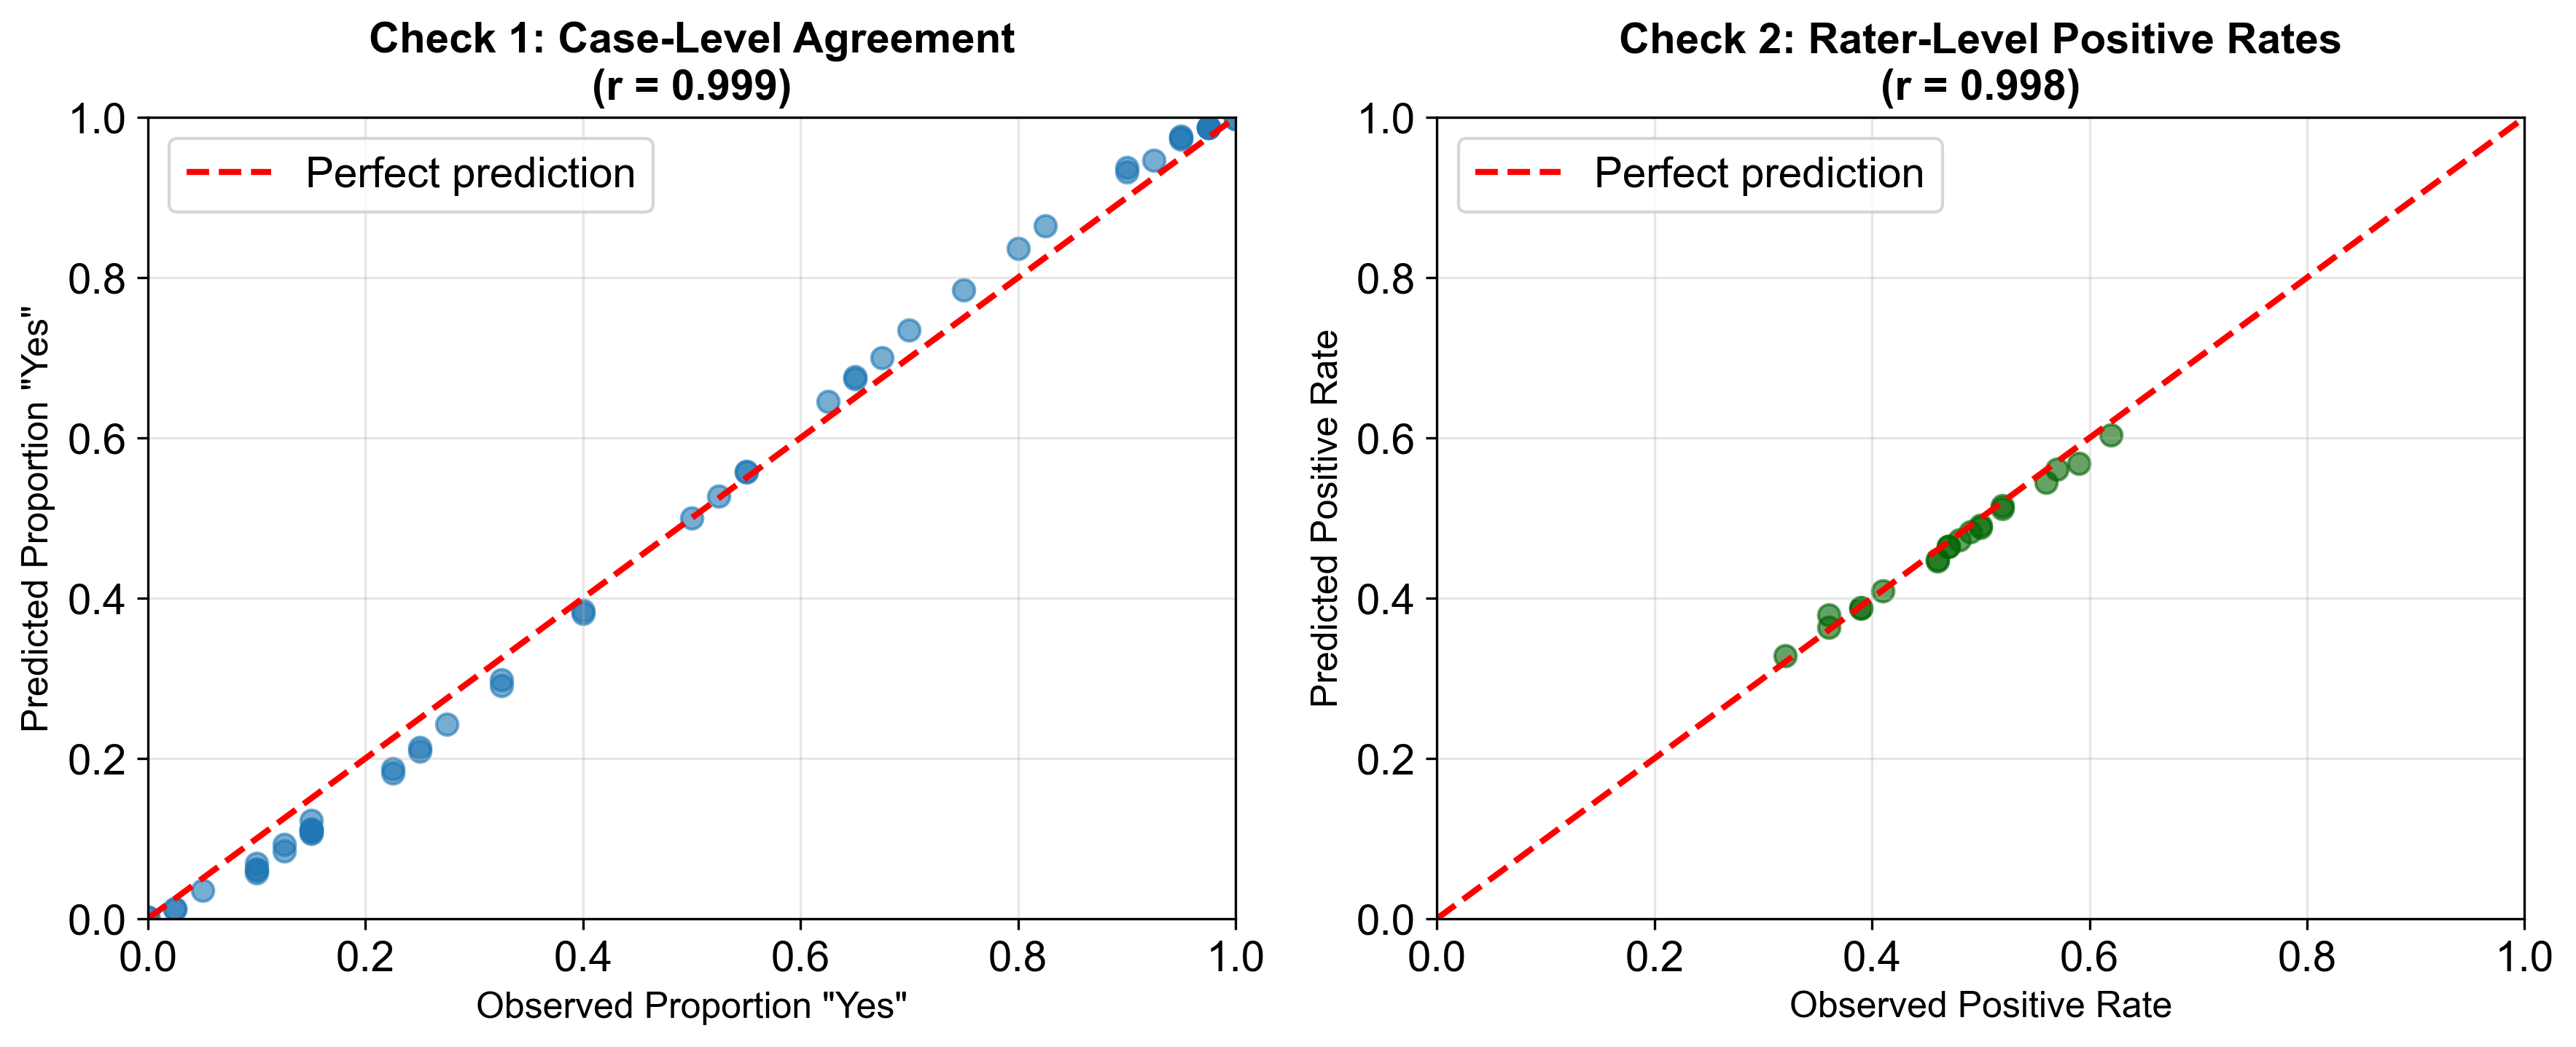
\includegraphics[width=0.95\textwidth]{posterior_predictive_checks.png}
\caption{Posterior predictive checks for model validation. \textbf{Left panel:} Case-level agreement showing observed versus predicted proportion of affirmative diagnoses across 50 cases ($r = 0.999$). \textbf{Right panel:} Rater-level positive rates showing observed versus predicted diagnostic rates across 20 experts ($r = 0.998$). Points cluster tightly along the diagonal (red dashed line) in both panels, confirming excellent model fit.}
\label{fig:ppc}
\end{figure}
